\documentclass[hyperref={pdfpagelabels=false}]{beamer}
\setbeamercolor{background canvas}{bg=white}
\usepackage{graphicx,lmodern,subfigure,ulem,color,graphicx,tikz,booktabs,natbib}
\usepackage{mathrsfs}
\usetheme{Warsaw}
%\definecolor{beamer@blendedblue}{rgb}{0.1,0.5,0.1}
%\definecolor{ForestGreen}{RGB}{60, 140, 60}
%\setbeamercolor{structure}{fg=beamer@blendedblue}
\setbeamertemplate{navigation symbols}{}
\setbeamertemplate{footline}[frame number]
\bibliographystyle{chicago}
\newcommand{\spitem}{\vspace{.3cm}\item}
\newcommand{\elas}{$E_{labor}$}
\def \ourFigPath {../../} 

\usetheme[
outer/progressbar=foot,
outer/numbering=none
]{metropolis}



\title{Project}
\author{Marco Brianti\\Vito Cormun}
\institute{Boston College}
\date{November 2018}


\begin{document}
	
	\frame{
		
		
		\maketitle
}



\frame{\frametitle{Objective of the Project}
	
	\
	
	Estimating responses of key macroeconomic variables to a sentiment shock.
	
	\
	
	\
	
	\textbf{Preview of the results:}
	
	\begin{enumerate}
		\item Most of the variables display a boom-bust response with peaks respectively at 2 and 10 quarters.  
		\item Effects on inflation are robustly nonsignificant or negative. 
	\end{enumerate}
	
     
    
    \
    
    \
    
    
		
}
	

\frame{\frametitle{Econometric Procedure - Overview}
	
	We use a 2-step procedure
	
	\
	
	\begin{enumerate}
		\item Estimate series of sentiment shocks using forecast revisions
		
		\
		
		\item Estimate IRFs via local projection \`a la Jorda (2005)
	\end{enumerate}
	
}


\frame{\frametitle{Step 1 - Overview}
	
	We estimate sentiment shocks as SPF forecast revisions of real GDP growth rate which are orthogonal to 
	
	\
	
		\begin{enumerate}
		\item contemporaneous structural shocks
		
		\
		
		\item lagged principal components from a large dataset
		
		\
		
		\item past and future TFP
	\end{enumerate}
	
}


\frame{\frametitle{Step 1 - Estimation of $Z_t$}
	
	Data 
	\begin{itemize}
	 \item $X_t$ is log of Real GDP at time $t$
	 \item $X_{t+k|t} = E[X_{t+k}|I_t]$ provided by SPF
	 \end{itemize}
 
 \
 
 Procedure
	$$
	Z_t = (X_{t+4|t} - X_{t|t}) - (X_{t+4|t-1} - X_{t|t-1})
	$$
	where 
	\begin{itemize}
	\item $(X_{t+4|t} - X_{t|t})$ is expected growth rate of Real GDP conditional on information set up to time $t$
	\item $(X_{t+4|t-1} - X_{t|t-1})$ is expected growth rate of Real GDP conditional on information set up to time $t-1$
	\item $Z_t$ is an innovation to the expectations of output growth rate
	\end{itemize}
}


\frame{\frametitle{Step 1 - Estimation of $\tilde{Z}_t$}
	\textbf{Problem.} ${Z}_t$ is correlated with current and future fundamentals such as fiscal policy, monetary policy, current and future TFP.
	
	\
	
	\textbf{Solution.} Estimate $\tilde{Z}_t$ as the residual of the following regression,	
$$
Z_t = C +  \sum_{j=-J}^H \delta_j \Delta TFP_{t+j} + \gamma SS_t + \mu PC_{t-1} + \tilde{Z}_t
$$
where
\begin{itemize}
	\item $C$ is a constant parameter
	\item $\Delta TFP_t$ is first difference of utility-adjusted total factor productivity at time $t$
	\item $SS_t$ is a vector of structural shocks at time $t$ possibly estimated via narrative approach
	\item $PC_{t-1}$ is a vector of principal component at time $t-1$
\end{itemize}

\

$\tilde{Z}_t$ represents a change in expectations which is orthogonal to any source of fundamental fluctuations, i.e. a \textbf{noise shock}.
	
}




\frame{\frametitle{Noise Shocks $\tilde{Z_t}$}
	
	\begin{center}
	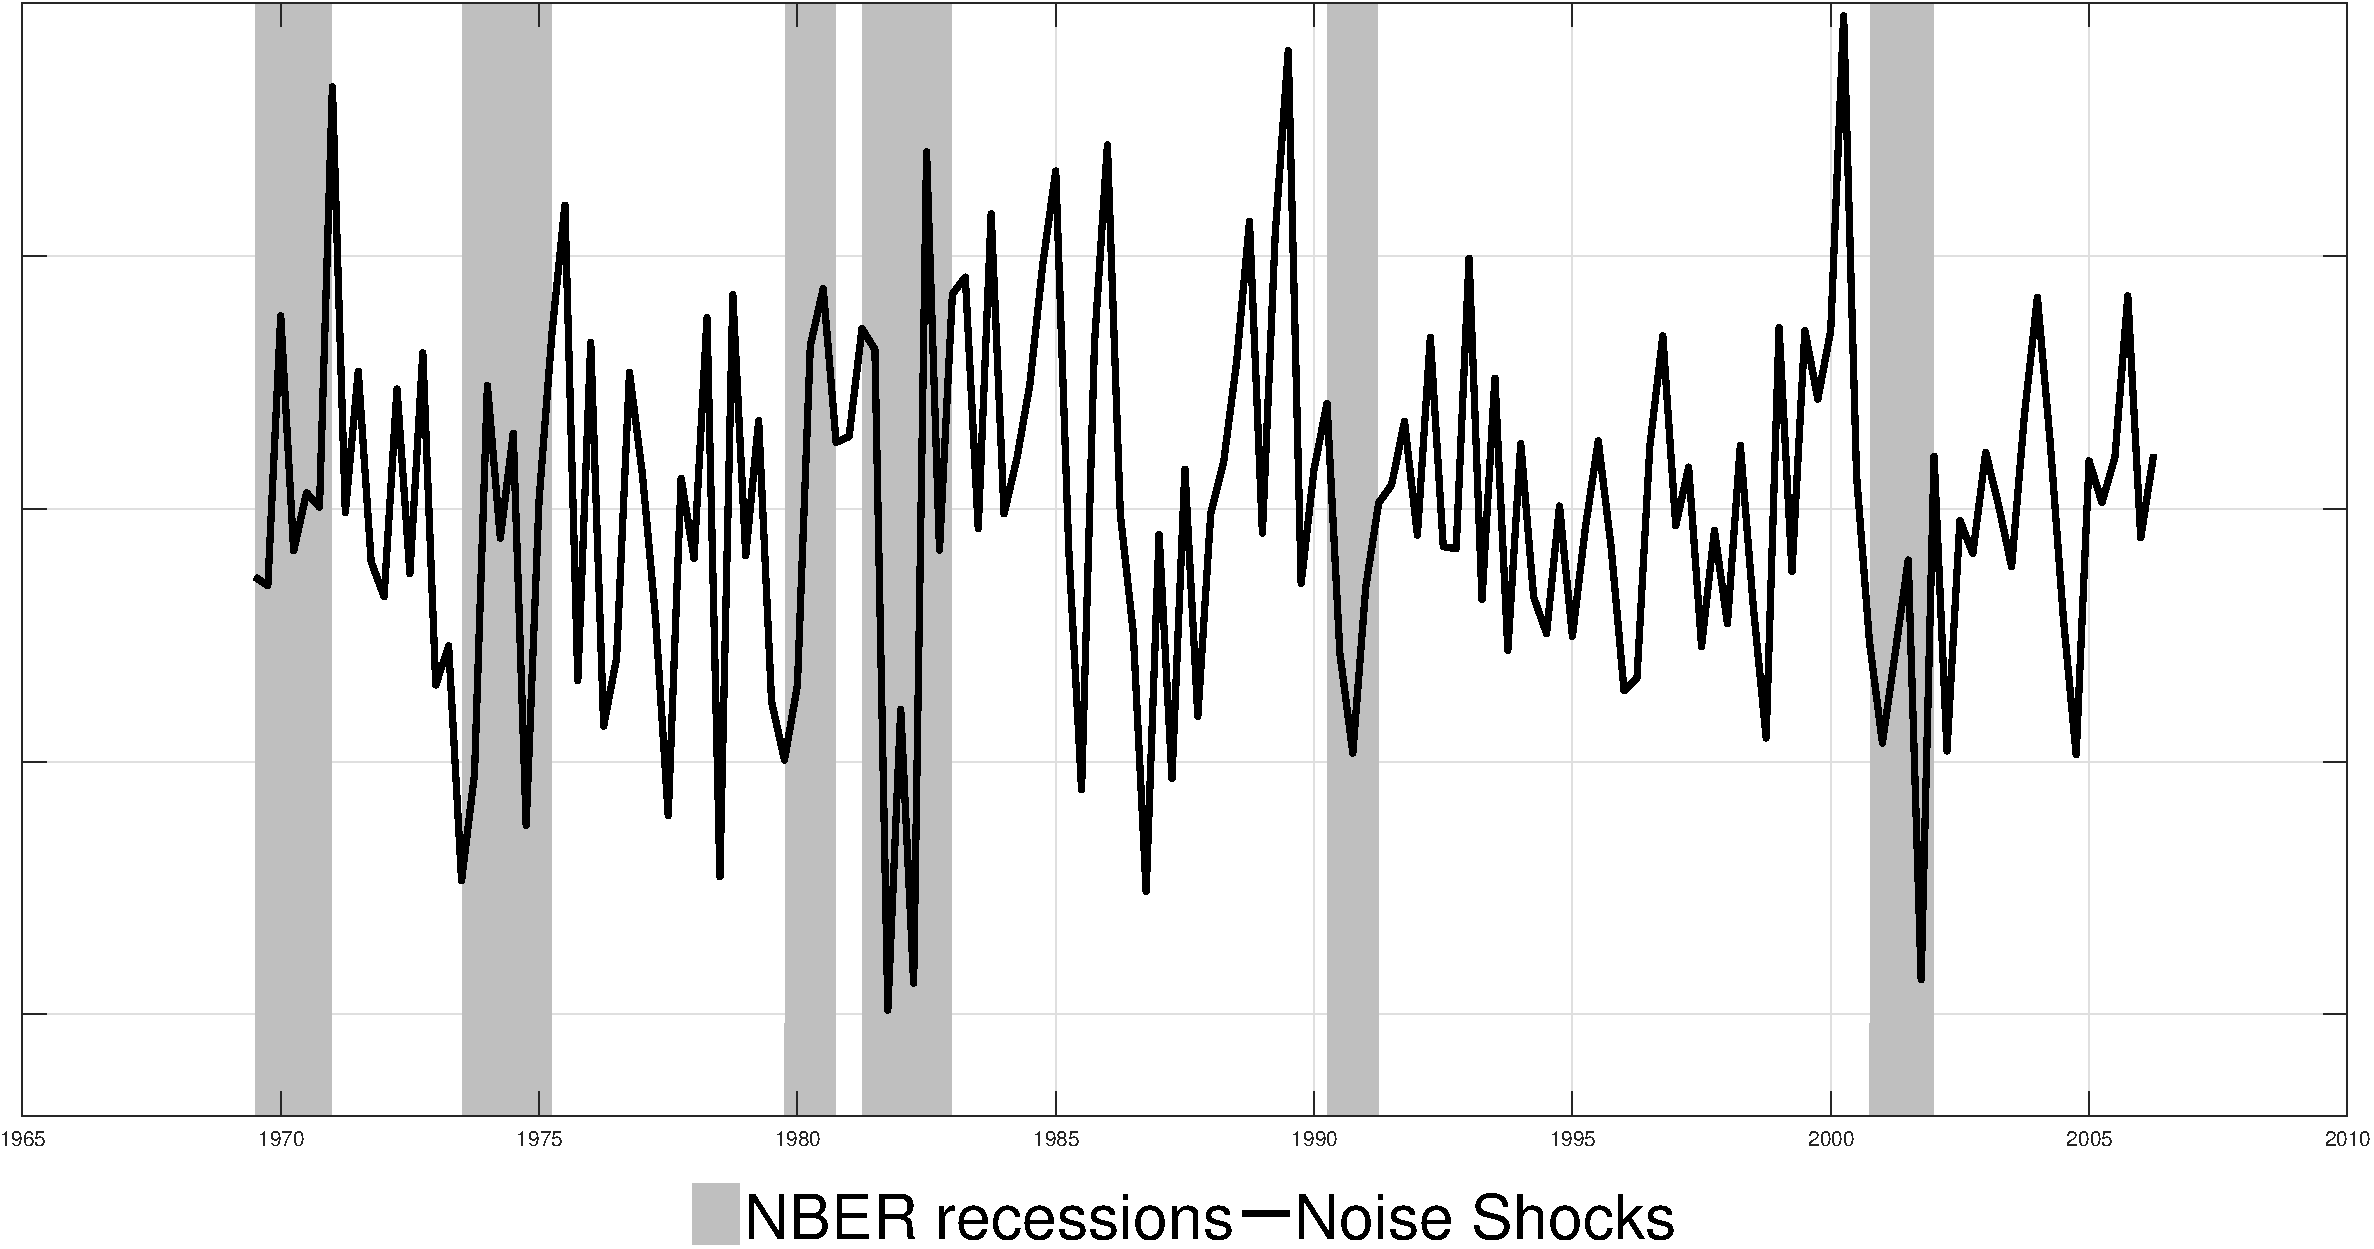
\includegraphics[scale = 0.27]{\ourFigPath Figures/Noise_Shocks_SPF_GDPgrowth_revisions}
\end{center}

}


\frame{\frametitle{Step 2 - Estimation of IRFs to $\tilde{Z}_t$}
	Define $Y_t$ to be the BP-filtered log-transformation of an endogenous aggregate macroeconomic variable.
	
	\
	
	Using standard OLS techniques we estimate $H$ regressions	
	$$
	Y_{t+h} = \Theta_h^Y \tilde{Z}_t + \epsilon_{t+h}
	$$
	where $h = 1,2, \dots, H$ represent the forecast horizon.

	
	\
	
$\Theta_1^Y, \ \Theta_2^Y, \ \dots, \ \Theta_H^Y$ represent the path of the impulse response function of $Y_t$ to a unit deviation of $\tilde{Z}_t$.
	
}

\frame{\frametitle{Bootstrapping Techniques}
	
	\begin{enumerate}
		 

	
\item Consider the tuple $\Gamma^Y_h = \{ Y_{t+h}, \ T_t, \ \tilde{Z}_t, \ X_{t-1} \}$.

\

\item Divide $\Gamma^Y_h$ over time $t$ in smaller blocks and randomly reorder these blocks in order to form a new tuple $\Gamma^Y_{h,Boot1}$ of the same size of the previous one.

\


\item Estimate $\Theta_{h,Boot1}$ from $\Gamma^Y_{h,Boot1}$ using standards OLS techniques.

\

\item Redo (1)-(3) $2000$ times and select confidence intervals.

	\end{enumerate}	
	
}

\frame{\frametitle{Local Projection - Confidence Interval 68\% and 90\%}
	
	\begin{center}
		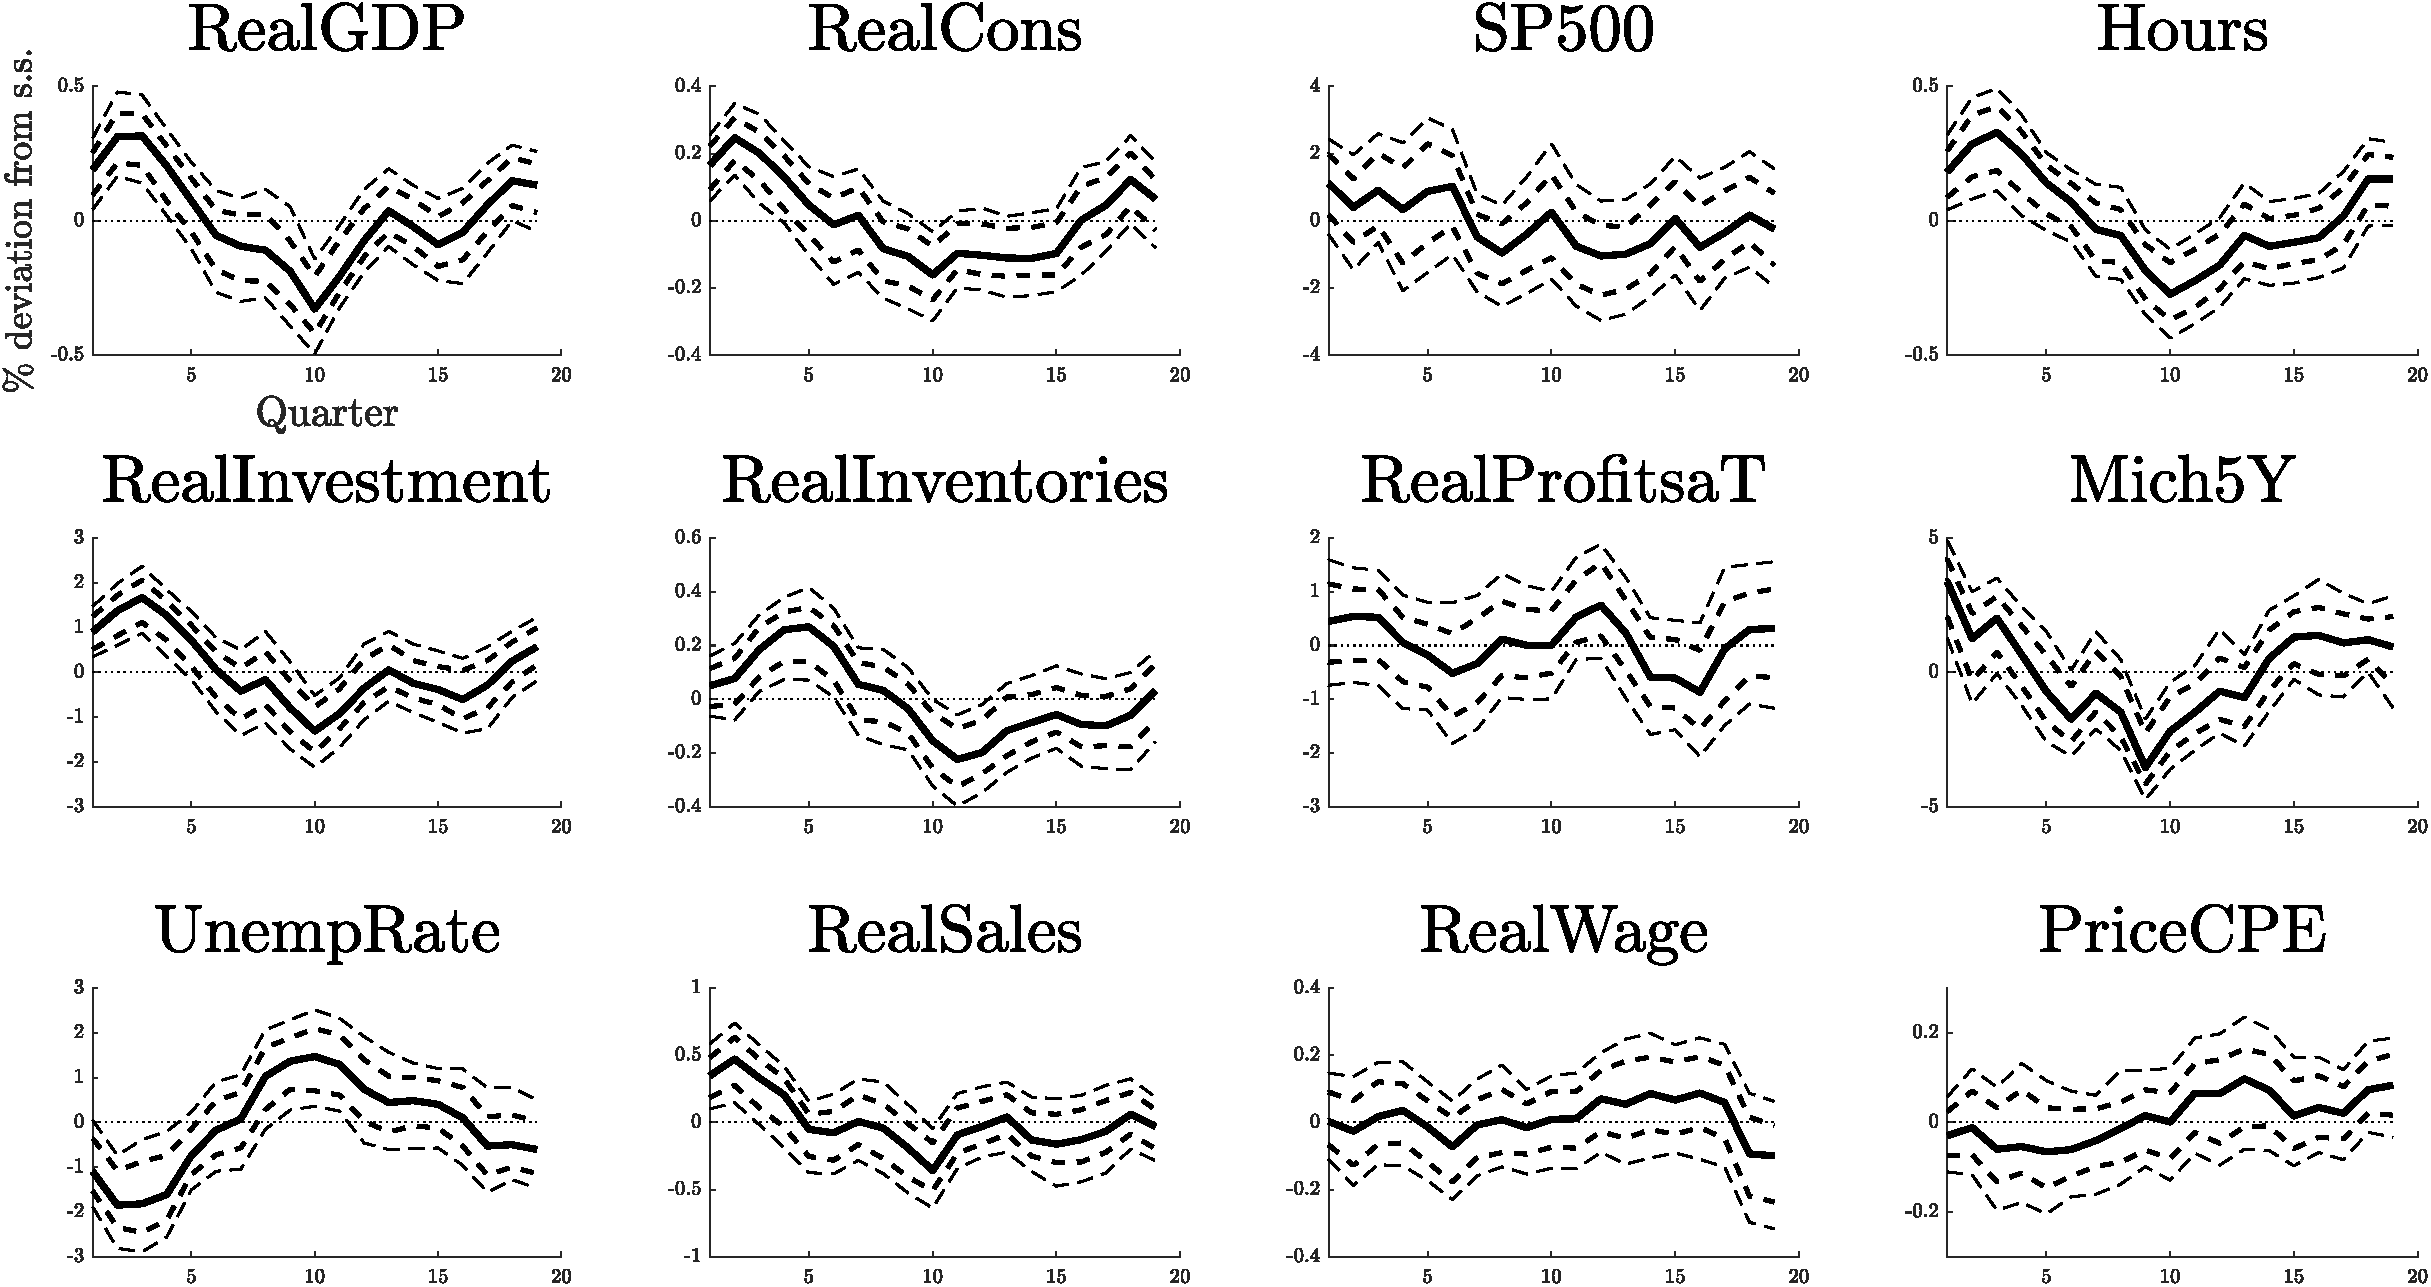
\includegraphics[scale = 0.27]{\ourFigPath Figures/MarcoVito_Nov272018_FigureRyanMeeting}
	\end{center}
	
	
}

\frame{\frametitle{Local Projection - Confidence Interval 68\% and 90\%}
	
	\begin{center}
		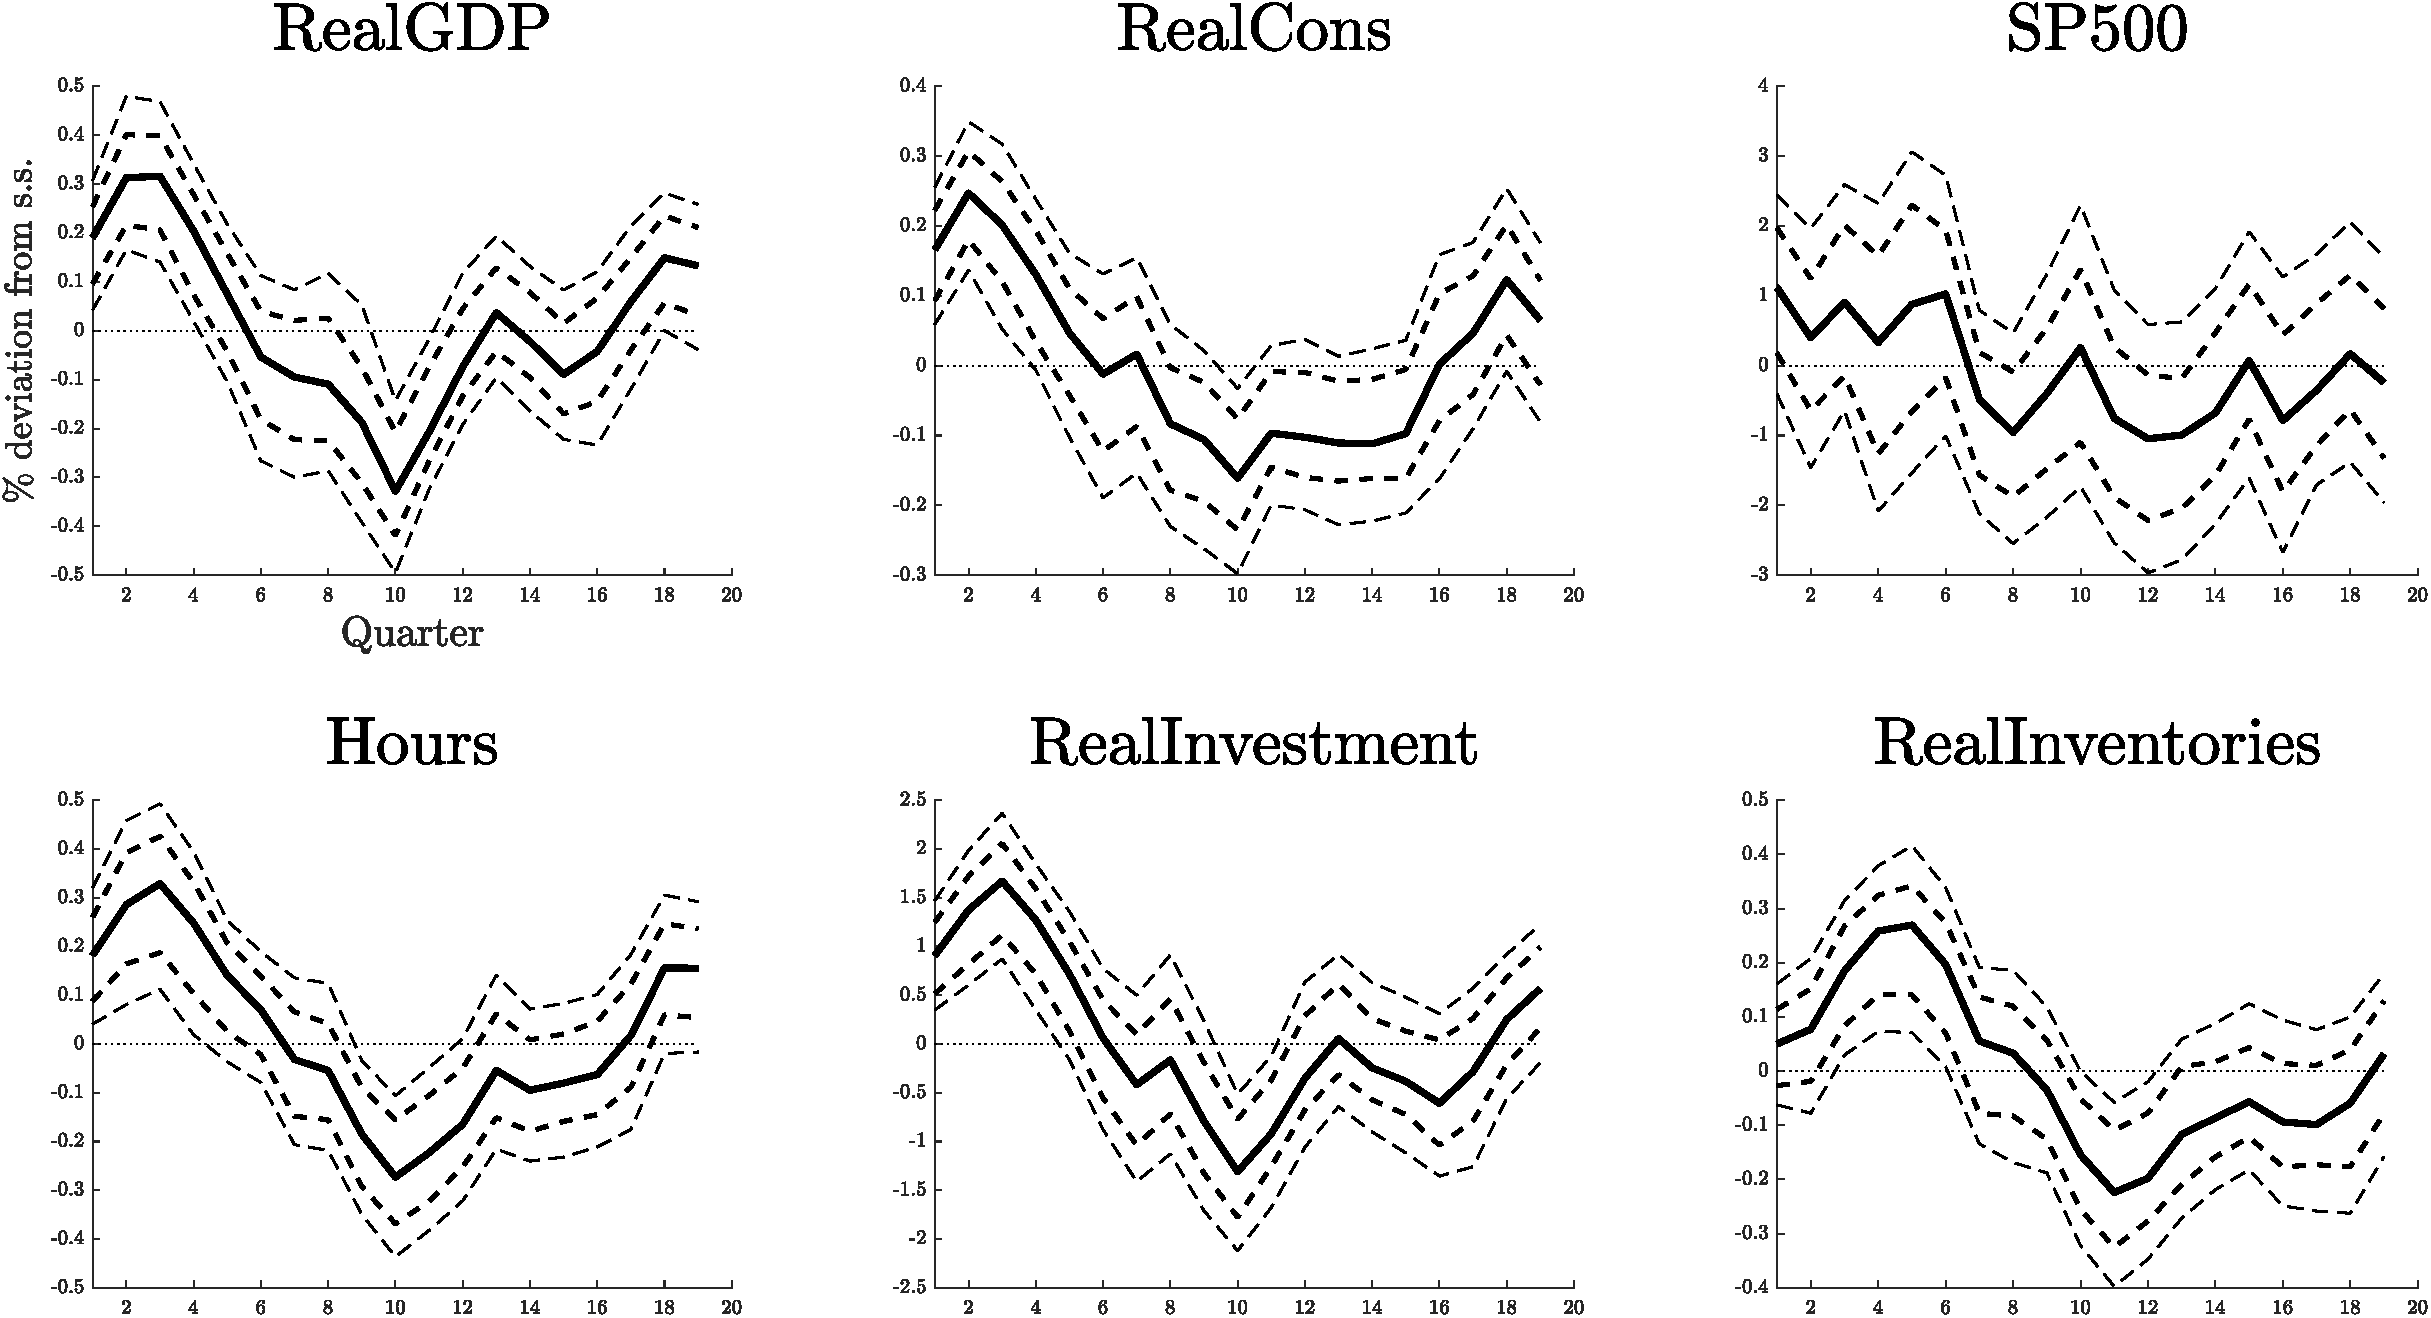
\includegraphics[scale = 0.27]{\ourFigPath Figures/MarcoVito_Nov272018_FigureRyanMeeting_Part1}
	\end{center}
	
	
}

\frame{\frametitle{Local Projection - Confidence Interval 68\% and 90\%}
	
	\begin{center}
		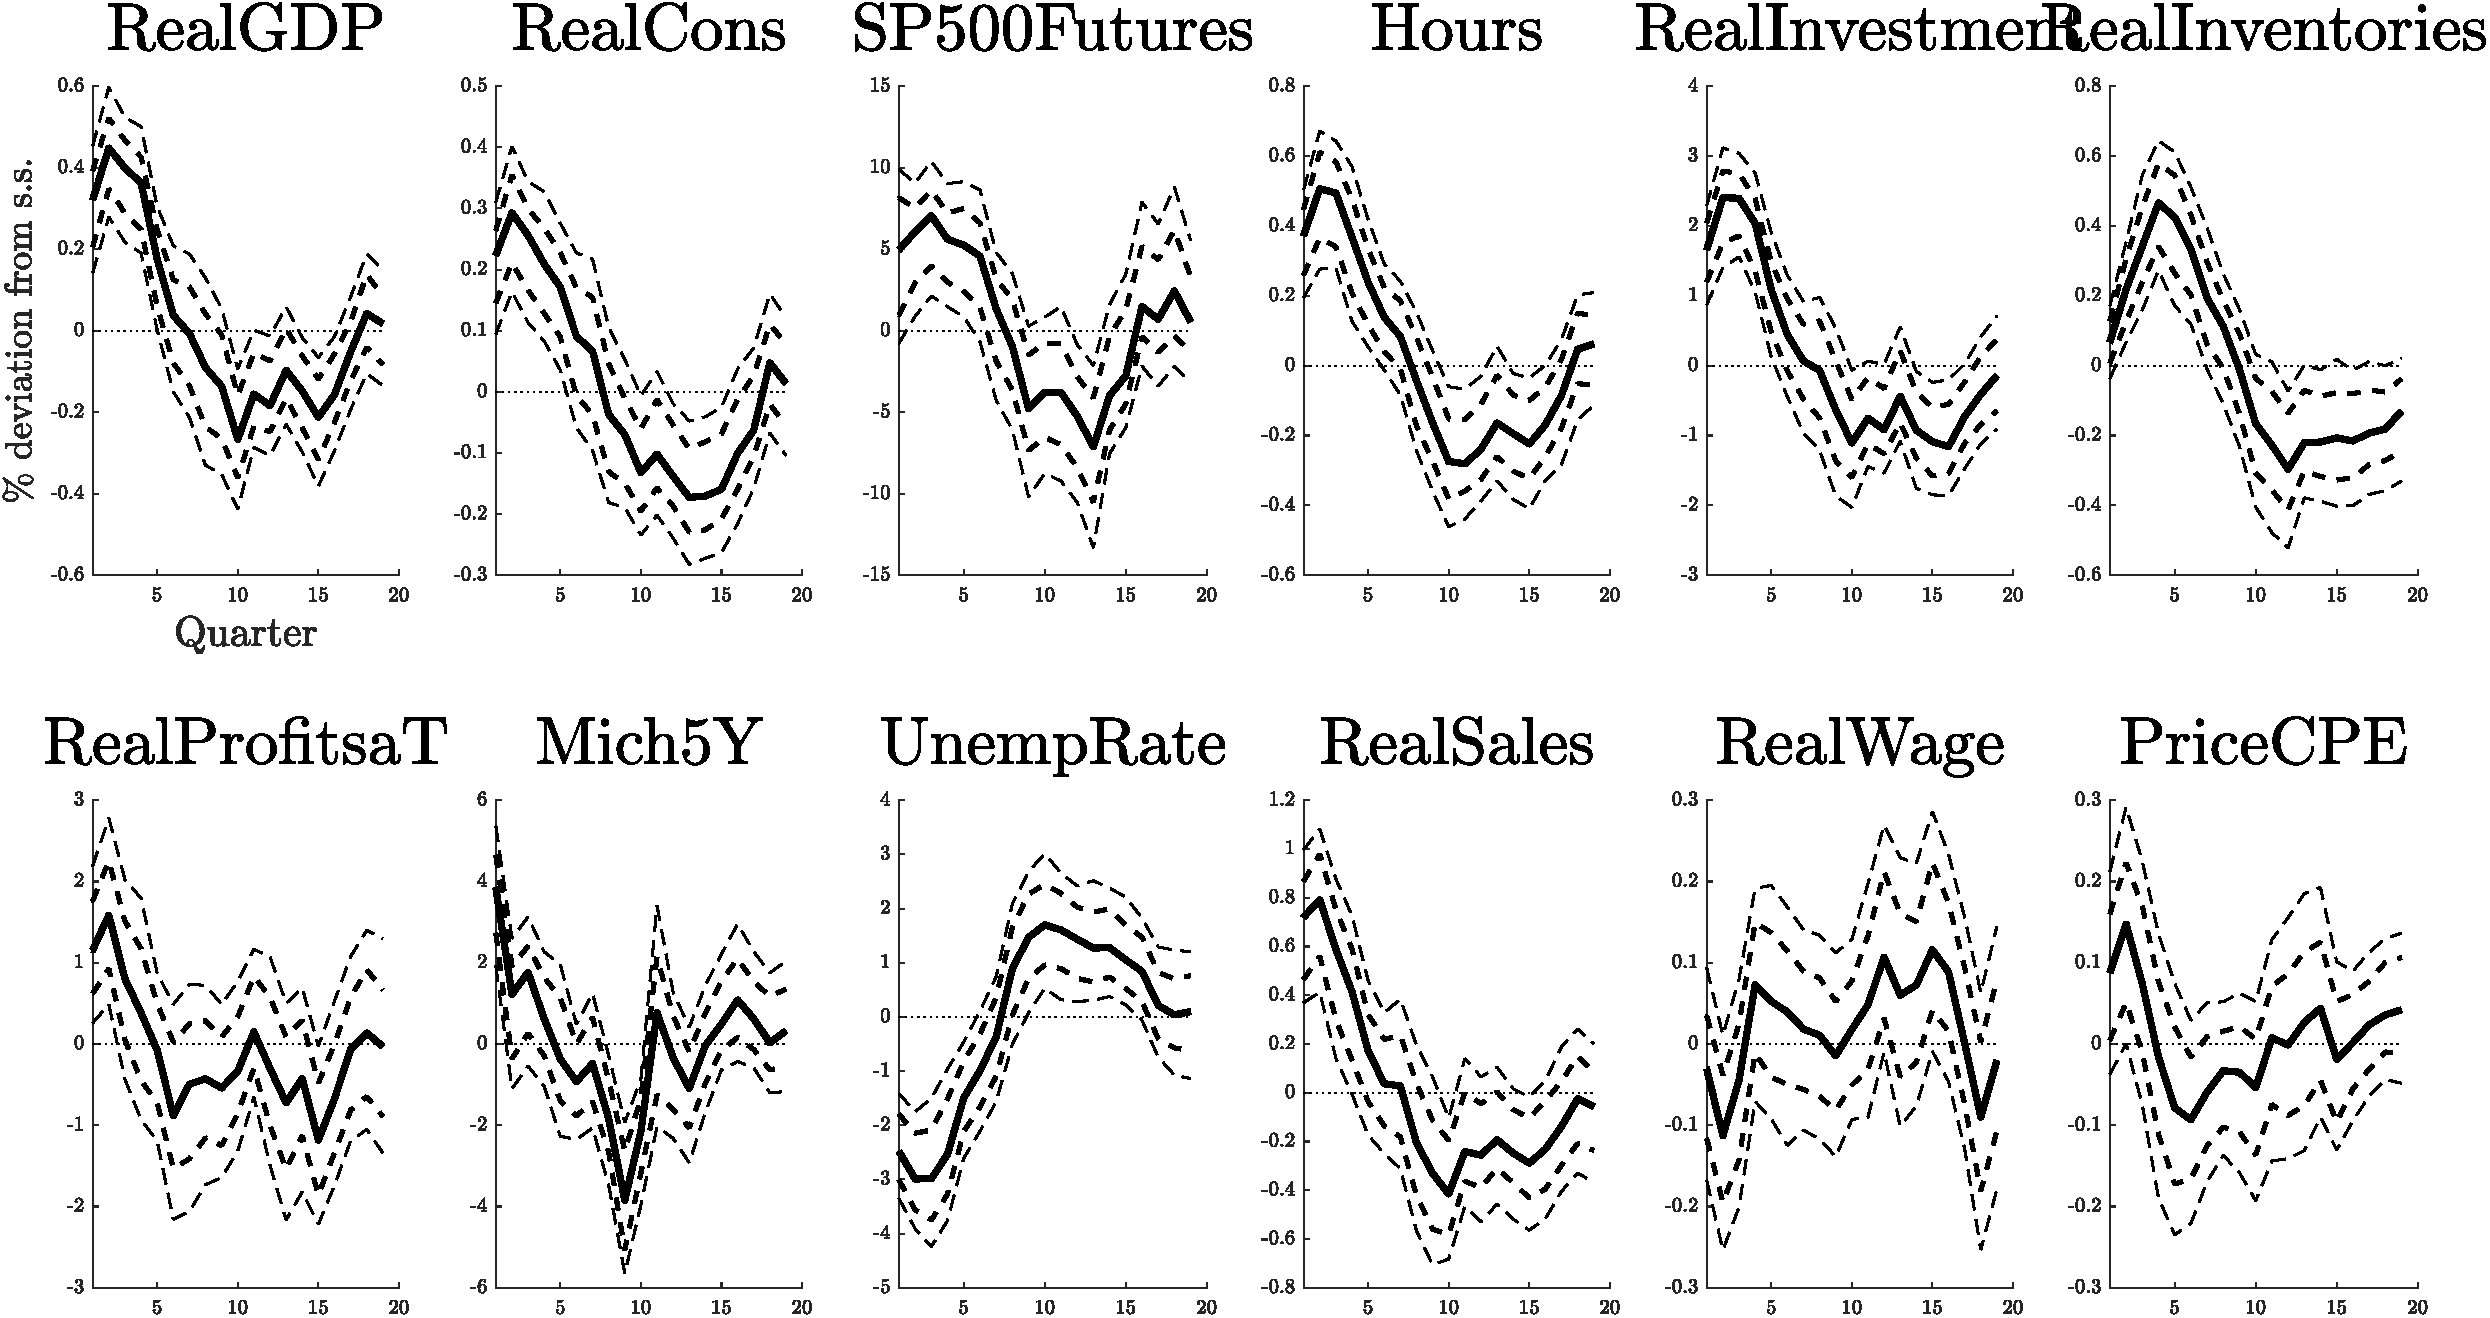
\includegraphics[scale = 0.27]{\ourFigPath Figures/MarcoVito_Nov272018_FigureRyanMeeting_Part2}
	\end{center}
	
	
}

\frame{\frametitle{Next}
	
\begin{enumerate}
	\item Discuss relation with existing literature 
	\begin{itemize}
		\item Typically sentiment shocks are identified as those orthogonal to TFP surprise and news shocks. These restrictions need not to hold (CJ). In fact our shock is correlated with news shocks.
		\item Discipline the literature on boom and bust: news that do not materialize vs sunspot. Our results are consistent mostly with the latter due to inventory behaviour (Crouzet and Oh). However, we need to empirically and theoretically investigate the role of non rational expectations.
		\end{itemize}
	\vskip 10pt
	\item Write a model. How specific? Ideally we would like the model to provide additional testable implications. We could use IBES data to extract expectation (error) at the firm level.
\end{enumerate}
	
}













\end{document}